%\input{preamble.txt}
%
%\begin{document}
\section{I/O and Regular Expressions}

\begin{itemize}
	\item Input and Output (I/O)
	\begin{itemize}
		\begin{minipage}[t]{\widthof{Input sources include:} + 1cm}
			\item Input sources include:
			\begin{itemize}
				\item Keyboard
				\item File
				\item Network
			\end{itemize}
		\end{minipage}
		\begin{minipage}[t]{\widthof{Output destinations include:} + 1cm}
			\item Output destinations include:
			\begin{itemize}
				\item Console
				\item File
				\item Network
			\end{itemize}
		\end{minipage}
	\end{itemize}

	\item Input and Output Streams
	\begin{itemize}
		\item Java handles inputs and outputs using streams\\
		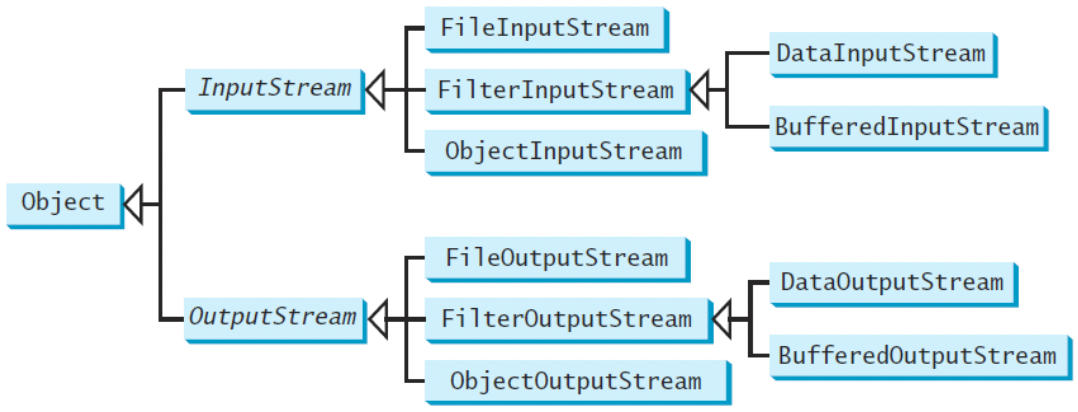
\includegraphics[scale=0.6]{IOChart}
	\end{itemize}

	\item Standard I/O
	\begin{itemize}
		\item \textbf{System.in}
		\begin{itemize}
			\item Object of type \textbf{InputStream}
			\item Typically refers to the keyboard
			\item Reading data could be done using the \textbf{Scanner} class. Its methods include:
			\begin{itemize}
				\begin{minipage}{\widthof{String nextLine()} + 1cm}
					\item \textbf{String next()}
					\item \textbf{String nextLine()}
				\end{minipage}
				\begin{minipage}{\widthof{double nextDouble()} + 1cm}
					\item \textbf{int nextInt()}
					\item \textbf{double nextDouble()}
				\end{minipage}
			\end{itemize}
		\end{itemize}

		\item \textbf{System.out}
		\begin{itemize}
			\item Object of type \textbf{PrintStream}
			\item Typically refers to the console
		\end{itemize}
	\end{itemize}

	\item The \textbf{File} class
	\begin{itemize}
		\item Contains methods for obtaining the properties of a file/directory and
		for renaming and deleting a file/directory
		\item Files could be specified using absolute or relative names
		\item Constructing a \textbf{File} instance does not create a file on the machine
		\item Methods include:
		\begin{itemize}
			\begin{minipage}[t]{\widthof{\textbf{boolean createNewFile()}} + 1cm}
				\item \textbf{boolean createNewFile()}
				\item \textbf{boolean delete()}
				\item \textbf{boolean exists()}
			\end{minipage}
			\begin{minipage}[t]{\widthof{\textbf{boolean isDirectory()}} + 1cm}
				\item \textbf{boolean isDirectory()}
				\item \textbf{File [] listFiles()}
			\end{minipage}
		\end{itemize}
	\end{itemize}

	\item File I/O
	\begin{itemize}
		\item Reading could be done using the \textbf{Scanner} class
		\begin{itemize}
			\item e.g. \textbf{Scanner input = new Scanner(new File(filename));}
		\end{itemize}
		\item Writing could be done using the \textbf{FileWrite} class
		\begin{itemize}
			\item e.g. \textbf{FileWriter output = new FileWriter(filename, append);}
		\end{itemize}
	\end{itemize}

	\newpage

	\item Regular Expressions
	\begin{itemize}
		\item A regular expression (abbreviated regex) is a string that describes a pattern for matching a set of strings.
		\item Regular expressions provide a simple and effective way to validate user input
		\begin{itemize}
			\item e.g. phone numbers
		\end{itemize}
		\item Java supports regular expressions using the \textbf{java.util.regex} package
		\item The \textbf{Pattern} class can be used to define the pattern
		\begin{itemize}
			\item The \textbf{compile} method takes a string representing the regular expression as an argument and compiles it into a pattern
		\end{itemize}
		\item The \textbf{Matcher} class can be used to search for the pattern. Its methods include:
		\begin{itemize}
			\item \textbf{boolean find()}
			\item \textbf{boolean matches()}
		\end{itemize}
		\item Example
		\begin{Verbatim}
	Pattern pattern = Pattern.compile("H.*d");
	Matcher matcher = pattern.matcher("Hello World");
	System.out.println(matcher.matches());
		\end{Verbatim}
	\end{itemize}

	\item Commonly Used Regular Expressions\\
	\begin{tabular}{l l l}
		\hline
		\textit{Regular Expression} & \textit{Matches} & \textit{Example}\\
		\hline
		\hline
		\texttt{.} & any single character & \texttt{Java} matches \texttt{J..a}\\
		\texttt{(ab|cd)} & \texttt{ab} or \texttt{cd} & \texttt{ten} matches \texttt{t(en|im)}\\
		\texttt{[abc]} & \texttt{a}, \texttt{b}, or \texttt{c} & \texttt{Java} matches \texttt{Ja[uvwx]a}\\
		\texttt{[\string^abc]} & any character except \texttt{a}, \texttt{b}, or \texttt{c} & \texttt{Java} matched \texttt{Ja[\string^ars]a}\\
		\texttt{[a-z]} & \texttt{a} through \texttt{z} & \texttt{Java} matches \texttt{[A-M]av[a-d]}\\
		\texttt{[\string^a-z]} & any character except \texttt{a} through \texttt{z} & \texttt{Java} matches \texttt{J]av[\string^b-d]}\\
		\texttt{[a-e[m-p]]} & \texttt{a} through \texttt{e} or \texttt{m} through \texttt{p} & \texttt{Java} matches \texttt{[A-G[I-M]]av[a-d]}\\
		\texttt{[a-e\&\&[c-p]] }& intersection of \texttt{a-e} with \texttt{c-p} & \texttt{Java} matches \texttt{[A-P\&\&[I-M]]av[a-d]}\\
		\texttt{\textbackslash d} & a digit, same as \texttt{[0-9]} & \texttt{Java2} matches ``\texttt{Java[\textbackslash\textbackslash d]}'' \\
		\texttt{\textbackslash D} & a non-digit & \texttt{\$Java} matches ``\texttt{[\textbackslash\textbackslash D][\textbackslash\textbackslash D]ava}"\\
		\texttt{\textbackslash w} & a word character & \texttt{Java1} matches ``\texttt{[\textbackslash\textbackslash w]ava[\textbackslash\textbackslash w]}"\\
		\texttt{\textbackslash W} & a non-word character & \texttt{\$Java } matches ``\texttt{[\textbackslash\textbackslash W][\textbackslash\textbackslash w]ava}"\\
		\texttt{\textbackslash s} & a whitespace character & ``\texttt{Java 2}'' matches ``\texttt{Java\textbackslash\textbackslash s2}"\\
		\texttt{\textbackslash S} & a non-whitespace character & \texttt{Java} matches ``\texttt{[\textbackslash\textbackslash S]ava}"\\
		\hline
		\texttt{\emph{p*}} & zero or more occurrences of pattern \texttt{\emph{p}} & \makecell[cc]{\texttt{aaaabb} matches ``\texttt{a*bb}" \\ \texttt{ababab} matches ``\texttt{(ab)*}"}\\
		\hline
		\texttt{\emph{p+}} & one or more occurrences of pattern \texttt{\emph{p}} & \makecell[cc]{\texttt{a} matches ``\texttt{a+b*}" \\ \texttt{able} matches ``\texttt{(ab)+.*}"}\\
		\hline
		\texttt{\emph{p?}} & zero or one occurrence of pattern \texttt{\emph{p}} & \makecell[cc]{\texttt{Java} matches ``\texttt{J?Java}" \\ \texttt{Java} matches ``\texttt{J?ava}"}\\
		\hline
		\texttt{\emph{p\{n\}}} & exactly \texttt{n} occurrences of pattern \texttt{\emph{p}} & \makecell[cc]{\texttt{Java} matches ``\texttt{J\{1\}.*}" \\ \texttt{Java} does not match ``\texttt{.\{2\}}"}\\
		\hline
		\texttt{\emph{p\{n,\}}} & at least \texttt{n} occurrences of pattern \texttt{\emph{p}} & \makecell[cc]{\texttt{aaaa} matches ``\texttt{a\{1,\}}" \\ \texttt{a} does not match ``\texttt{a\{2,\}}"}\\
		\hline
		\texttt{\emph{p\{n, m\}}} & between \texttt{n} and \texttt{m} occurrences (inclusive) & \makecell[cc]{\texttt{aaaa} matches ``\texttt{a\{1,9\}}" \\ \texttt{abb} does not match ``\texttt{a\{2,9\}bb}"}\\
	\end{tabular}

\end{itemize}


%\end{document}